% Construction : droite graduée de -0.6 à 5.4, entiers en 0..5.
%   x = 3.4, plancher ⌊x⌋ = 3, successeur 4. Le crochet marque [3 ; 4[.
% SVG : x = 30 + 46x, y = 70 (axe).
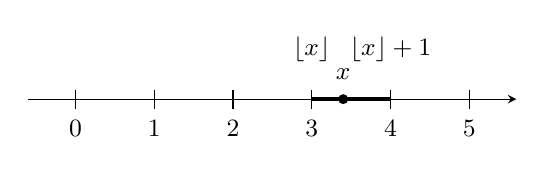
\begin{tikzpicture}[scale=1, >=stealth, every node/.style={font=\small}]
  \draw[->] (-0.6, 0) -- (5.6, 0);
  \foreach \n in {0,1,2,3,4,5} { \draw (\n, 0.12) -- (\n, -0.12); \node[below] at (\n, -0.15) {$\n$}; }
  \draw[very thick] (3, 0) -- (4, 0);
  \fill (3.4, 0) circle (1.8pt);
  \node[above] at (3.4, 0.12) {$x$};
  \node[above] at (3, 0.35) {$\lfloor x \rfloor$};
  \node[above] at (4, 0.35) {$\lfloor x \rfloor + 1$};
\end{tikzpicture}
